\chapter{Zuur-base-evenwichten en de methode van de predominante reactie}\label{ch:b1:predominant-reaction}

Azijn lost de kalkaanslag van een waterkoker op; citroensap ook, en iets
sneller. Bloed houdt zijn pH binnen nauwe grenzen, wat we ook eten; een
frisdrank met prik is zuur door het koolstofdioxide dat erin opgelost is.
Het zijn allemaal zuur-base-evenwichten in water, en een chemicus die
voor een oplossing met meerdere zuren en basen staat --- een mengsel, een
buffer, een \omterm{def:b1:predominant-reaction:polyprotic}{meerwaardig zuur} --- heeft een betrouwbare manier nodig om
haar pH en de concentraties van haar deeltjes te vinden. Dit hoofdstuk
bouwt die methode op: een sterkteschaal, \omterm{def:b1:predominant-reaction:predominance}{predominantiediagrammen}, en de
\emph{methode van de \omterm{def:b1:predominant-reaction:predominant-reaction}{predominante reactie}}, die elk mengsel terugbrengt
tot de ene reactie die ertoe doet.

\begin{recall}
Boek 1 (jaar 12) definieerde zuren en basen volgens Brønsted, de
\omterm{def:b1:predominant-reaction:acidity-constant}{zuurconstante} $K_a$ en de $\mathrm{p}K_a$, het \omterm{def:b1:predominant-reaction:autoprotolysis}{ionenproduct van water} en
de pH van \omterm{def:b1:predominant-reaction:strong-acid}{sterke zuren} en basen, en tekende \omterm{def:b1:predominant-reaction:predominance}{predominantiediagrammen}. Het
\omterm{def:b1:extent-q-and-k:quotient}{reactiequotiënt}, de evenwichtsconstante en de \omterm{def:b1:extent-q-and-k:activity}{activiteiten} van opgeloste
stoffen ($c/c^\circ$) en van het oplosmiddel (1) werden gedefinieerd in
\cref{ch:b1:extent-q-and-k}; in dit hoofdstuk wordt $c^\circ = \qty{1}{mol/L}$ niet in de quotiënten geschreven.
\end{recall}

\begin{omfigure}
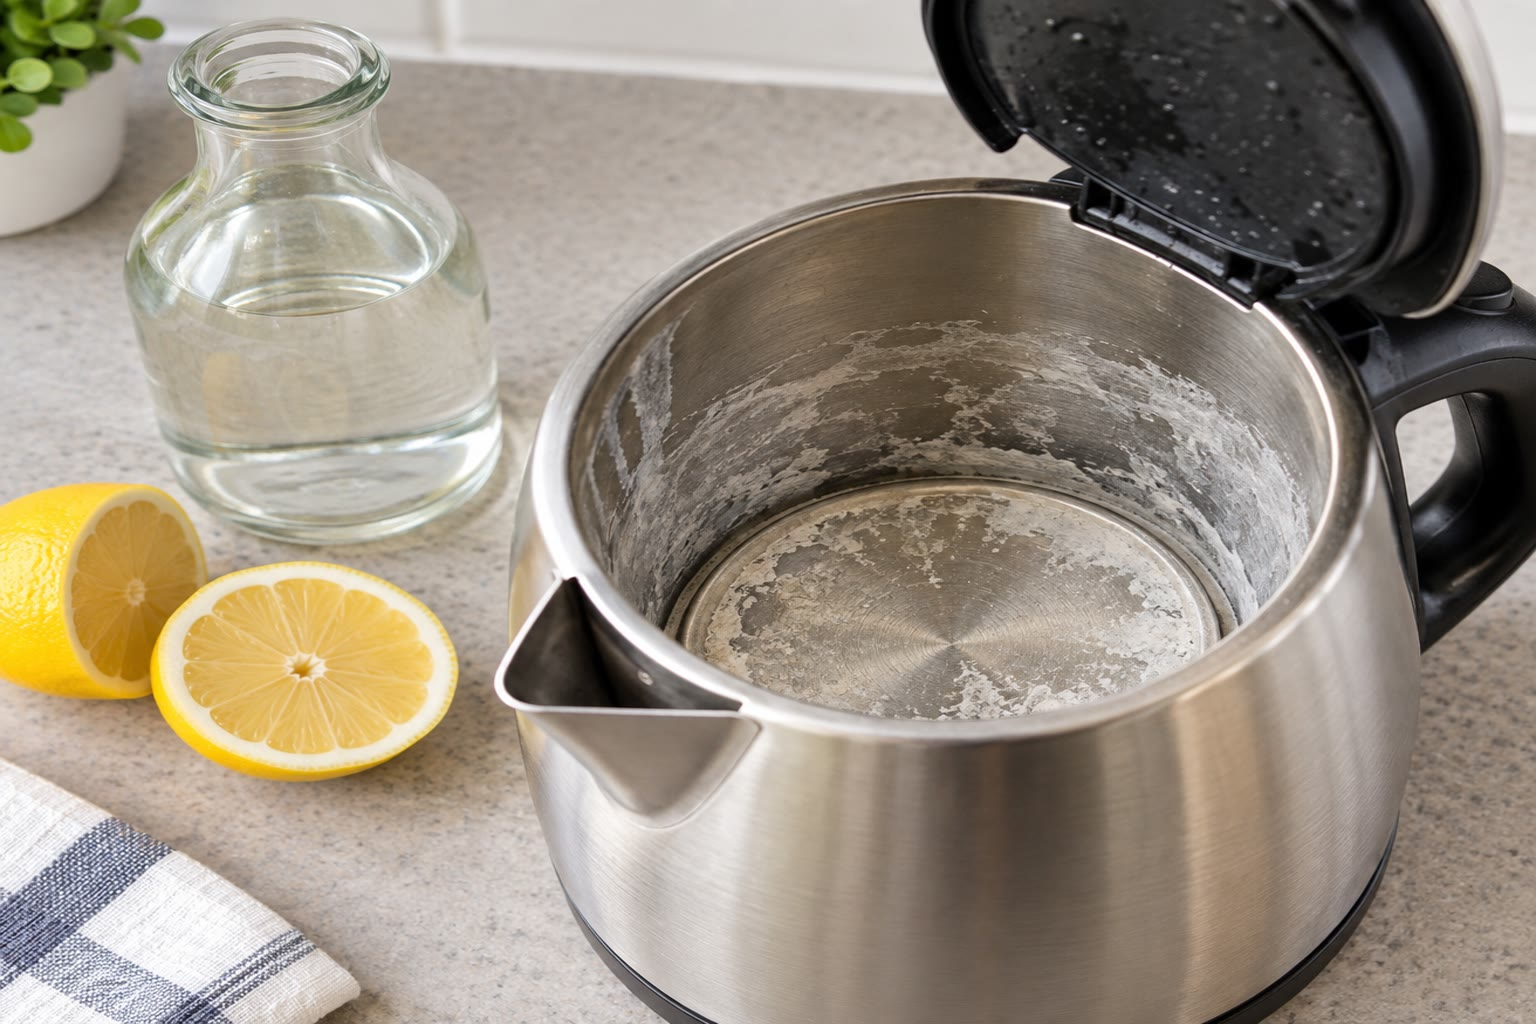
\includegraphics[width=0.5\linewidth]{images/book2/ai/b1-10-descaling.jpg}

{\small Kalkaanslag, calciumcarbonaat, in een waterkoker. De \omterm{def:b1:predominant-reaction:strong-acid}{zwakke
zuren} van azijn en citroensap reageren met het carbonaation en lossen het
op.}
\end{omfigure}

\section{Koppels volgens Brønsted en de pH}

\begin{definition}[Zuur en base volgens Brønsted, koppel]\label{def:b1:predominant-reaction:bronsted}
Een \emph{zuur volgens Brønsted}\index{zuur volgens Bronsted@zuur volgens Brønsted}
is een deeltje dat een proton \ce{H+} kan afstaan; een \emph{base volgens
Brønsted}\index{base volgens Bronsted@base volgens Brønsted} is een
deeltje dat er een kan opnemen. Een zuur HA en de base A die het wordt
door een proton te verliezen, vormen een
\emph{zuur-basekoppel}\index{zuur-basekoppel} HA/A, verbonden door de
formele halfreactie $\mathrm{HA} \rightleftharpoons
\mathrm{A} + \ce{H+}$. In water is het proton nooit vrij: het wordt door
een watermolecuul gedragen als \ce{H3O+}.
\end{definition}

\begin{definition}[Amfolyt]\label{def:b1:predominant-reaction:ampholyte}
Een \emph{amfolyt}\index{amfolyt} (een amfoteer deeltje) is de base van
het ene koppel en het zuur van een ander: water (\ce{H3O+}/\ce{H2O} en
\ce{H2O}/\ce{OH-}), het waterstofcarbonaation (\ce{CO2,H2O}/\ce{HCO3-}
en \ce{HCO3-}/\ce{CO3^{2-}}), het diwaterstoffosfaation.
\end{definition}

\begin{definition}[Autoprotolyse, ionenproduct, pH]\label{def:b1:predominant-reaction:autoprotolysis}
Water ondergaat \emph{autoprotolyse}\index{autoprotolyse},
\ce{2H2O <=> H3O+ + OH-}, met constante $K_e = [\ce{H3O+}][\ce{OH-}]$, het
\emph{ionenproduct van water}\index{ionenproduct van water}; bij
\qty{25}{\celsius} is $K_e = 10^{-14.00}$, dus $\mathrm{p}K_e = 14.00$. De
pH van een oplossing is $\mathrm{pH} = -\log a(\ce{H3O+}) \approx -\log[\ce{H3O+}]$.
Een oplossing is neutraal wanneer $[\ce{H3O+}] = [\ce{OH-}]$, dus bij
$\mathrm{pH} = \mathrm{p}K_e/2 = 7.00$ bij \qty{25}{\celsius}.
% ledger: dfg:H2O_l, dfg:OH-_ao (pKe computed in figdata/bachelor-1/aqueous-constants.py)
\end{definition}


\section{Sterkte: \texorpdfstring{$K_a$}{Ka}, \texorpdfstring{p$K_a$}{pKa} en het nivellerende effect}

\begin{definition}[Zuurconstante]\label{def:b1:predominant-reaction:acidity-constant}
De \emph{zuurconstante}\index{zuurconstante} van een koppel HA/A is de
constante van de reactie van het zuur met water,
\[
  \mathrm{HA} + \ce{H2O} \rightleftharpoons \mathrm{A} + \ce{H3O+}, \qquad
  K_a = \frac{[\mathrm{A}][\ce{H3O+}]}{[\mathrm{HA}]}, \qquad
  \mathrm{p}K_a = -\log K_a .
\]
Hoe groter $K_a$ (hoe kleiner $\mathrm{p}K_a$), hoe sterker het zuur en
hoe zwakker zijn geconjugeerde base.
\end{definition}

\begin{definition}[Sterke en zwakke zuren en basen]\label{def:b1:predominant-reaction:strong-acid}
Een zuur is in water \emph{sterk}\index{sterk zuur} als zijn reactie met
water aflopend is: er blijft geen enkel molecuul HA over (zoutzuur,
salpeterzuur, perchloorzuur, de eerste zuurfunctie van zwavelzuur);
anders is het \emph{zwak}\index{zwak zuur}. Een base is
\emph{sterk}\index{sterke base} als haar reactie met water aflopend is en
\ce{OH-} geeft (hydroxiden, het oxide-ion, alkoxiden), en anders
\emph{zwak}\index{zwakke base}.
\end{definition}

\begin{definition}[Nivellerend effect]\label{def:b1:predominant-reaction:levelling}
In water reageert elk zuur dat sterker is dan \ce{H3O+} volledig tot
\ce{H3O+}, en elke base die sterker is dan \ce{OH-} volledig tot
\ce{OH-}: hun sterkten zijn niet te onderscheiden. Dat is het
\emph{nivellerende effect}\index{nivellerend effect} van het
oplosmiddel. \omterm{def:b1:predominant-reaction:strong-acid}{Zwakke zuren} en basen in water hebben
$0 < \mathrm{p}K_a < 14$, waarbij de koppels van water zelf
($\mathrm{p}K_a(\ce{H3O+}/\ce{H2O}) = 0$ en
$\mathrm{p}K_a(\ce{H2O}/\ce{OH-}) = 14$) de schaal begrenzen.
\end{definition}

\begin{center}
\small
\begin{tabular}{lll@{\hspace{2.5em}}lll}
\hline
koppel & p$K_a$ & & koppel & p$K_a$ & \\
\hline
\ce{HSO4-}/\ce{SO4^{2-}} & 1.99 & & \ce{CO2,H2O}/\ce{HCO3-} & 6.37 & \\
\ce{H3PO4}/\ce{H2PO4-} & 2.15 & & \ce{H2PO4-}/\ce{HPO4^{2-}} & 7.21 & \\
\ce{HF}/\ce{F-} & 3.16 & & \ce{HClO}/\ce{ClO-} & 7.55 & \\
\ce{HCOOH}/\ce{HCOO-} & 3.74 & & \ce{NH4+}/\ce{NH3} & 9.25 & \\
\ce{CH3COOH}/\ce{CH3COO-} & 4.76 & & \ce{C6H5OH}/\ce{C6H5O-} & 9.99 & \\
\ce{C6H5NH3+}/\ce{C6H5NH2} & 4.60 & & \ce{HCO3-}/\ce{CO3^{2-}} & 10.33 & \\
\ce{C6H5COOH}/\ce{C6H5COO-} & 4.21 & & \ce{CH3NH3+}/\ce{CH3NH2} & 10.66 & \\
\hline
\end{tabular}
\end{center}
% ledger: pka:methanoic, pka:ethanoic, pka:anilinium, pka:benzoic,
% pka:phenol, pka:methylammonium (IUPAC dataset); dfg:HSO4-_ao,
% dfg:SO42-_ao, dfg:H3PO4_ao, dfg:H2PO4-_ao, dfg:HPO42-_ao, dfg:HF_ao,
% dfg:F-_ao, dfg:CO2_ao, dfg:HCO3-_ao, dfg:CO32-_ao, dfg:HClO_ao,
% dfg:ClO-_ao, dfg:NH4+_ao, dfg:NH3_ao (pKa computed from NBS-82)


\section{Predominantie- en verdelingsdiagrammen}

\begin{definition}[Predominantie- en verdelingsdiagrammen]\label{def:b1:predominant-reaction:predominance}
Voor een koppel HA/A is $\mathrm{pH} = \mathrm{p}K_a + \log([\mathrm{A}]/[\mathrm{HA}])$:
het zuur overheerst ($[\mathrm{HA}] > [\mathrm{A}]$) voor
$\mathrm{pH} < \mathrm{p}K_a$, de base voor $\mathrm{pH} > \mathrm{p}K_a$.
Het \emph{predominantiediagram}\index{predominantiediagram} is de pH-as,
bij elke $\mathrm{p}K_a$ verdeeld in de gebieden waar elke vorm
overheerst. Het \emph{verdelingsdiagram}\index{verdelingsdiagram} geeft de
fractie van elke vorm, $[\text{vorm}]/C$, als functie van de pH.
\end{definition}

\begin{proposition}[De betrekking van Henderson en de fracties]\label{prop:b1:predominant-reaction:henderson}
Voor een koppel HA/A met totale concentratie $C = [\mathrm{HA}] + [\mathrm{A}]$
is
\[
  \mathrm{pH} = \mathrm{p}K_a + \log\frac{[\mathrm{A}]}{[\mathrm{HA}]}, \qquad
  \frac{[\mathrm{HA}]}{C} = \frac{1}{1 + 10^{\mathrm{pH} - \mathrm{p}K_a}}, \qquad
  \frac{[\mathrm{A}]}{C} = \frac{1}{1 + 10^{\mathrm{p}K_a - \mathrm{pH}}} .
\]
Eén pH-eenheid van $\mathrm{p}K_a$ verwijderd is de minder voorkomende
vorm onder 10\,\% van het totaal; twee eenheden verwijderd, onder 1\,\%.
\end{proposition}

\begin{proof}
Neem de logaritme van $K_a = [\mathrm{A}][\ce{H3O+}]/[\mathrm{HA}]$. Dan
is $[\mathrm{A}]/[\mathrm{HA}] = 10^{\mathrm{pH}-\mathrm{p}K_a}$, en delen
van $[\mathrm{HA}]$ door $[\mathrm{HA}] + [\mathrm{A}]$ geeft de fracties.
Bij $\mathrm{pH} = \mathrm{p}K_a + 1$ is $[\mathrm{HA}]/C = 1/11 < 10\,\%$;
bij $+2$, $1/101$.
\end{proof}

\begin{omfigure}
\begin{tikzpicture}
\begin{axis}[name=e,
  width=0.48\linewidth, height=5.2cm, xmin=0, xmax=14, ymin=0, ymax=1.05,
  axis x line=bottom, axis y line=left, xlabel={pH}, ylabel={fractie},
  xtick={0,2,4,6,8,10,12,14},
  tick label style={font=\small}, label style={font=\small}]
\addplot[omDef, thick] table[x=pH, y=HA] {figdata/out/bachelor-1-distribution-diagrams-ethanoic.dat};
\addplot[omThm, thick] table[x=pH, y=A] {figdata/out/bachelor-1-distribution-diagrams-ethanoic.dat};
\draw[dotted] (axis cs:4.76,0) -- (axis cs:4.76,0.5);
\node[omDef, font=\footnotesize, anchor=west] at (axis cs:0.3,0.3) {\ce{CH3COOH}};
\node[omThm, font=\footnotesize, anchor=east] at (axis cs:13.7,0.3) {\ce{CH3COO-}};
\node[font=\small, anchor=north west] at (axis cs:4.8,0.48) {4.76};
\end{axis}
\begin{axis}[at={(e.east)}, anchor=west, xshift=1.1cm,
  width=0.48\linewidth, height=5.2cm, xmin=0, xmax=14, ymin=0, ymax=1.05,
  axis x line=bottom, axis y line=left, xlabel={pH}, ylabel={fractie},
  xtick={0,2,4,6,8,10,12,14},
  legend style={font=\scriptsize, draw=none, at={(0.5,1.04)}, anchor=south, legend columns=4},
  tick label style={font=\small}, label style={font=\small}]
\addplot[omDef, thick] table[x=pH, y=H3A] {figdata/out/bachelor-1-distribution-diagrams-phosphoric.dat};
\addplot[omMeth, thick] table[x=pH, y=H2A] {figdata/out/bachelor-1-distribution-diagrams-phosphoric.dat};
\addplot[omProp, thick] table[x=pH, y=HA] {figdata/out/bachelor-1-distribution-diagrams-phosphoric.dat};
\addplot[omThm, thick] table[x=pH, y=A] {figdata/out/bachelor-1-distribution-diagrams-phosphoric.dat};
\legend{\ce{H3PO4}, \ce{H2PO4-}, \ce{HPO4^{2-}}, \ce{PO4^{3-}}}

\end{axis}
\end{tikzpicture}

\begin{tikzpicture}[font=\small, >={Stealth}]
  \draw[->, thick] (0,0) -- (14.2*0.85,0) node[right] {pH};
  \foreach \x/\l in {2.15/2.15, 7.21/7.21, 12.34/12.34}
    \draw (\x*0.85,0.15) -- (\x*0.85,-0.15) node[below] {\l};
  \node[above] at (1.07*0.85,0.1) {\ce{H3PO4}};
  \node[above] at (4.68*0.85,0.1) {\ce{H2PO4-}};
  \node[above] at (9.78*0.85,0.1) {\ce{HPO4^{2-}}};
  \node[above] at (13.3*0.85,0.1) {\ce{PO4^{3-}}};
\end{tikzpicture}

{\small \omterm{def:b1:predominant-reaction:predominance}{Verdelingsdiagrammen} van ethaanzuur (links) en fosforzuur
(rechts), en het \omterm{def:b1:predominant-reaction:predominance}{predominantiediagram} van fosforzuur. Elk snijpunt van
twee naburige krommen ligt bij een $\mathrm{p}K_a$; de \omterm{def:b1:predominant-reaction:ampholyte}{amfolyten}
\ce{H2PO4-} en \ce{HPO4^{2-}} zijn in het midden van hun gebied bijna de
enige vorm.}
\end{omfigure}

\section{De methode van de predominante reactie}

\begin{proposition}[Constante van een zuur-basereactie]\label{prop:b1:predominant-reaction:k-of-reaction}
De reactie van het zuur $\mathrm{HA}_1$ van een koppel met de base
$\mathrm{A}_2$ van een ander,
$\mathrm{HA}_1 + \mathrm{A}_2 \rightleftharpoons \mathrm{A}_1 + \mathrm{HA}_2$,
heeft de constante
\[
  K = \frac{K_{a1}}{K_{a2}} = 10^{\,\mathrm{p}K_{a2} - \mathrm{p}K_{a1}} .
\]
Ze is gunstig ($K > 1$) wanneer het zuur sterker is dan het zuur dat
ontstaat ($\mathrm{p}K_{a1} < \mathrm{p}K_{a2}$), en \omterm{def:b1:extent-q-and-k:quantitative}{kwantitatief} (in de
zin van \cref{met:b1:extent-q-and-k:quantitative}) wanneer het verschil
in $\mathrm{p}K_a$ groter is dan ongeveer 4.
\end{proposition}

\begin{proof}
De reactie is de som van $\mathrm{HA}_1 + \ce{H2O} \rightleftharpoons
\mathrm{A}_1 + \ce{H3O+}$ ($K_{a1}$) en van de omgekeerde reactie van
$\mathrm{HA}_2 +
\ce{H2O} \rightleftharpoons \mathrm{A}_2 + \ce{H3O+}$ ($1/K_{a2}$);
\cref{prop:b1:extent-q-and-k:combine-k} geeft $K = K_{a1}/K_{a2}$.
\end{proof}

\begin{definition}[Predominante reactie, equivalente oplossing]\label{def:b1:predominant-reaction:predominant-reaction}
In een oplossing met meerdere zuren en basen is de \emph{predominante
reactie}\index{predominante reactie} de reactie met de grootste
constante, tussen het sterkste zuur en de sterkste base die aanwezig
zijn. Als ze \omterm{def:b1:extent-q-and-k:quantitative}{kwantitatief} is, wordt ze als aflopend behandeld, en wordt
de oplossing vervangen door de \emph{equivalente
oplossing}\index{equivalente oplossing}: de oplossing die ontstaat zodra
deze reactie voltooid is, en die dezelfde pH heeft als de echte.
\end{definition}

\begin{method}[De methode van de predominante reactie]\label{met:b1:predominant-reaction:method}
Zo bepaal je de pH en de samenstelling van een oplossing:
\begin{enumerate}
  \item som de ingebrachte deeltjes op (en water) en plaats hun koppels
        op een $\mathrm{p}K_a$-schaal, zuren aan de ene kant, basen aan de
        andere;
  \item zoek het sterkste zuur en de sterkste base die aanwezig zijn;
  \item is de constante van hun reactie groot ($K > 10^4$, of
        $\Delta\mathrm{p}K_a > 4$), behandel de reactie dan als aflopend
        en schrijf de \omterm{def:b1:predominant-reaction:predominant-reaction}{equivalente oplossing} op; ga terug naar stap 2;
  \item heeft de \omterm{def:b1:predominant-reaction:predominant-reaction}{predominante reactie} een kleine constante, dan bepaalt
        zij de pH: stel haar voortgangstabel op en los $Q = K$ op, meestal
        met de hypothese dat haar voortgang klein is;
  \item controleer de hypothesen: de minder voorkomende deeltjes zijn
        inderdaad klein in hoeveelheid, en de andere reacties (ook de
        \omterm{def:b1:predominant-reaction:autoprotolysis}{autoprotolyse} van water) zijn verwaarloosbaar.
\end{enumerate}
\end{method}

\begin{omfigure}
\begin{tikzpicture}[font=\small, >={Stealth}]
  \draw[->, thick] (0,-0.3) -- (0,7.6) node[above] {p$K_a$};
  \foreach \y/\a/\b in {0/\ce{H3O+}/\ce{H2O}, 1.58/\ce{HF}/\ce{F-}, 2.38/\ce{CH3COOH}/\ce{CH3COO-},
      3.62/\ce{H2PO4-}/\ce{HPO4^{2-}}, 4.62/\ce{NH4+}/\ce{NH3}, 7/\ce{H2O}/\ce{OH-}} {
    \draw (-0.12,\y) -- (0.12,\y);
    \node[anchor=east] at (-0.2,\y) {\a};
    \node[anchor=west] at (0.2,\y) {\b};
  }
  \foreach \y/\l in {0/0, 1.58/3.16, 2.38/4.76, 3.62/7.21, 4.62/9.25, 7/14} \node[black!60, anchor=west] at (3.0,\y) {\l};
  \draw[->, omThm, thick] (-1.6,2.55) -- (1.2,4.45);
  \node[omThm, anchor=west, align=left] at (4.2,3.5) {een zuur reageert met elke\\base die erboven staat: $K > 1$};
  \node[anchor=south] at (-1.4,7.35) {zuren};
  \node[anchor=south] at (1.2,7.35) {basen};
\end{tikzpicture}

{\small Een $\mathrm{p}K_a$-schaal (getekend met p$K_a$ naar boven
toenemend; waarden rechts). Een zuur reageert gunstig met elke base die
er op de schaal boven staat: hier ethaanzuur met ammoniak,
$K = 10^{9.25 - 4.76} = 10^{4.49}$.}
\end{omfigure}

\begin{proposition}[pH van eenvoudige oplossingen]\label{prop:b1:predominant-reaction:ph-formulas}
Bij concentratie $C$ (in \unit{mol/L}), met $\mathrm{p}C = -\log C$:
\begin{itemize}
  \item \omterm{def:b1:predominant-reaction:strong-acid}{sterk zuur}: $\mathrm{pH} = \mathrm{p}C$, geldig voor
        $\mathrm{pH} < 6.5$;
  \item \omterm{def:b1:predominant-reaction:strong-acid}{zwak zuur}, weinig gedissocieerd: $\mathrm{pH} = \frac12(\mathrm{p}K_a
        + \mathrm{p}C)$, geldig als $\mathrm{pH} < \mathrm{p}K_a - 1$;
  \item \omterm{def:b1:predominant-reaction:strong-acid}{zwakke base}, weinig geprotoneerd: $\mathrm{pH} = \frac12(\mathrm{p}K_e +
        \mathrm{p}K_a - \mathrm{p}C)$, geldig als $\mathrm{pH} > \mathrm{p}K_a +
        1$;
  \item \omterm{def:b1:predominant-reaction:ampholyte}{amfolyt} met $\mathrm{p}K_{a2} - \mathrm{p}K_{a1} > 4$:
        $\mathrm{pH} = \frac12(\mathrm{p}K_{a1} + \mathrm{p}K_{a2})$,
        ongeacht $C$ (mits niet te verdund).
\end{itemize}
\end{proposition}

\begin{proof}
\omterm{def:b1:predominant-reaction:strong-acid}{Sterk zuur}: \ce{HA + H2O -> A- + H3O+} is aflopend, $[\ce{H3O+}] = C$,
waarbij de eigen bijdrage van water ($10^{-7}$) verwaarloosbaar is als
$C > 10^{-6.5}$. \omterm{def:b1:predominant-reaction:strong-acid}{Zwak zuur}: de \omterm{def:b1:predominant-reaction:predominant-reaction}{predominante reactie} is $\mathrm{HA} + \ce{H2O}
\rightleftharpoons \mathrm{A} + \ce{H3O+}$ met voortgang $x = [\ce{H3O+}]
= [\mathrm{A}]$; als $x \ll C$, is $K_a = x^2/C$, $\mathrm{pH} = \frac12(\mathrm{p}K_a
+ \mathrm{p}C)$; de hypothese $[\mathrm{A}] < [\mathrm{HA}]/10$ komt neer op
$\mathrm{pH} < \mathrm{p}K_a - 1$. \omterm{def:b1:predominant-reaction:strong-acid}{Zwakke base}: hetzelfde met $\mathrm{A} +
\ce{H2O} \rightleftharpoons \mathrm{HA} + \ce{OH-}$, met constante $K_e/K_a$.
\omterm{def:b1:predominant-reaction:ampholyte}{Amfolyt} HA$^-$: de \omterm{def:b1:predominant-reaction:predominant-reaction}{predominante reactie} is $2\,\mathrm{HA}^- \rightleftharpoons
\mathrm{H_2A} + \mathrm{A}^{2-}$, dus $[\mathrm{H_2A}] = [\mathrm{A}^{2-}]$;
vermenigvuldigen van $K_{a1} = [\mathrm{HA}^-]h/[\mathrm{H_2A}]$ met $K_{a2} =
[\mathrm{A}^{2-}]h/[\mathrm{HA}^-]$ geeft $h^2 = K_{a1}K_{a2}$.
\end{proof}

\begin{omfigure}
\begin{tikzpicture}
\begin{axis}[
  width=0.66\linewidth, height=5.6cm, xmin=0, xmax=8, ymin=0, ymax=8,
  axis x line=bottom, axis y line=left,
  xlabel={$\mathrm{p}C = -\log C$}, ylabel={pH},
  xtick={0,1,2,3,4,5,6,7,8}, ytick={0,1,2,3,4,5,6,7,8},
  tick label style={font=\small}, label style={font=\small},
  legend style={font=\small, draw=none, at={(0.02,0.98)}, anchor=north west}]
\addplot[omDef, very thick] table[x=pC, y=pH] {figdata/out/bachelor-1-weak-acid-ph.dat};
\addplot[omProp, dashed] table[x=pC, y=weak] {figdata/out/bachelor-1-weak-acid-ph.dat};
\addplot[black!50, dotted, thick] table[x=pC, y=strong] {figdata/out/bachelor-1-weak-acid-ph.dat};
\draw[black!30] (axis cs:0,7) -- (axis cs:8,7);
\legend{exact, $\frac12(\mathrm{p}K_a + \mathrm{p}C)$, $\mathrm{pH} = \mathrm{p}C$}
\end{axis}
\end{tikzpicture}

{\small pH van oplossingen van ethaanzuur tegen $\mathrm{p}C$, exact
berekend uit de ladingsbalans. Geconcentreerd is het zuur weinig
gedissocieerd en volgt het $\frac12(\mathrm{p}K_a + \mathrm{p}C)$;
verdund tot onder ongeveer $10^{-6}$ mol/L is het volledig gedissocieerd
en gedraagt het zich als een \omterm{def:b1:predominant-reaction:strong-acid}{sterk zuur}; zeer verdund gaat de pH naar 7.}
\end{omfigure}

\begin{example}[Ethaanzuur en ammoniak]\label{ex:b1:predominant-reaction:mixture}
Meng \qty{0.10}{mol} ethaanzuur en \qty{0.10}{mol} ammoniak in
\qty{1.0}{L}. Het sterkste zuur is \ce{CH3COOH}, de sterkste base
\ce{NH3}: \ce{CH3COOH + NH3 <=> CH3COO- + NH4+}, $K = 10^{9.25 - 4.76} =
10^{4.49}$, \omterm{def:b1:extent-q-and-k:quantitative}{kwantitatief}. De \omterm{def:b1:predominant-reaction:predominant-reaction}{equivalente oplossing} bevat
\qty{0.10}{mol/L} \ce{CH3COO-} en \ce{NH4+}. Haar \omterm{def:b1:predominant-reaction:predominant-reaction}{predominante reactie},
\ce{NH4+ + CH3COO- <=> NH3 + CH3COOH}, heeft de kleine constante
$10^{-4.49}$ en houdt $[\ce{NH3}] = [\ce{CH3COOH}]$, waaruit, zoals voor
een \omterm{def:b1:predominant-reaction:ampholyte}{amfolyt}, $\mathrm{pH} = \frac12(4.76 + 9.25) = 7.01$ volgt.
\end{example}

\section{Polyprotische zuren en buffers}

\begin{definition}[Polyprotisch zuur]\label{def:b1:predominant-reaction:polyprotic}
Een \emph{polyprotisch zuur}\index{polyprotisch zuur} (of meerwaardig
zuur) kan na elkaar meerdere protonen afstaan, elke stap met zijn eigen
constante: fosforzuur \ce{H3PO4} ($\mathrm{p}K_a$ = 2.15, 7.21, 12.34),
koolzuur (\ce{CO2,H2O}; 6.37, 10.33), zwavelzuur (eerste zuurfunctie
sterk, tweede 1.99). De opeenvolgende $\mathrm{p}K_a$-waarden nemen toe:
een proton verwijderen uit een deeltje dat al negatief is, kost meer.
\end{definition}

\begin{example}[Fosforzuur bij \texorpdfstring{\qty{0.10}{mol/L}}{0.10 mol/L}]\label{ex:b1:predominant-reaction:h3po4}
De \omterm{def:b1:predominant-reaction:predominant-reaction}{predominante reactie} is de eerste zuurfunctie. Met $x = [\ce{H3O+}]$
is $x^2/(0.10 - x) = 10^{-2.15}$; hier is $x$ niet klein ten opzichte van
$C$, zodat de vierkantsvergelijking $x^2 + K_{a1}x - K_{a1}C = 0$ opgelost
wordt: $x =
\qty{0.0233}{mol/L}$, $\mathrm{pH} = 1.63$. De tweede zuurfunctie
($\mathrm{p}K_{a2} = 7.21$) draagt bij deze pH niets bij.
\end{example}

\begin{definition}[Bufferoplossing]\label{def:b1:predominant-reaction:buffer}
Een \emph{bufferoplossing}\index{bufferoplossing} is een oplossing
waarvan de pH weinig verandert wanneer een kleine hoeveelheid zuur of
base wordt toegevoegd, of wanneer ze verdund wordt. De gebruikelijke
buffer is een mengsel van een \omterm{def:b1:predominant-reaction:strong-acid}{zwak zuur} en zijn geconjugeerde base in
vergelijkbare hoeveelheden; haar pH ligt dicht bij de $\mathrm{p}K_a$ van
het koppel.
\end{definition}

\begin{proposition}[Waarom een buffer weerstand biedt]\label{prop:b1:predominant-reaction:buffer}
Voor een buffer van $n_a$ mol zuur en $n_b$ mol base hangt $\mathrm{pH} =
\mathrm{p}K_a + \log(n_b/n_a)$ niet af van het volume. Toevoegen van
$\delta$ mol van een \omterm{def:b1:predominant-reaction:strong-acid}{sterk zuur} verandert de pH met
\[
  \Delta\mathrm{pH} = \log\frac{n_b - \delta}{n_a + \delta} - \log\frac{n_b}{n_a}
  \approx -\frac{\delta}{\ln 10}\left(\frac{1}{n_a} + \frac{1}{n_b}\right),
\]
wat het kleinst is voor $n_a = n_b$ bij een gegeven totale hoeveelheid.
\end{proposition}

\begin{proof}
Het \omterm{def:b1:predominant-reaction:strong-acid}{sterke zuur} reageert volledig met de base: $n_b \to n_b - \delta$,
$n_a \to n_a + \delta$. De afgeleide van $f(\delta) = \log(n_b - \delta) -
\log(n_a + \delta)$ in 0 is $-\frac{1}{\ln10}\big(\frac{1}{n_b} +
\frac{1}{n_a}\big)$; bij vaste $n_a + n_b$ is $\frac1{n_a} + \frac1{n_b}$
het kleinst wanneer $n_a = n_b$.
\end{proof}

\begin{definition}[Dissociatiegraad]\label{def:b1:predominant-reaction:dissociation}
De \emph{dissociatiegraad}\index{dissociatiegraad} van een \omterm{def:b1:predominant-reaction:strong-acid}{zwak zuur} HA
met analytische concentratie $C$ is $\alpha = [\mathrm{A}]/C$, de fractie
van het zuur die door water gedissocieerd is; ze voldoet aan de
verdunningswet van Ostwald $\alpha^2C/(1 - \alpha) = K_a$, en gaat naar 1
als $C \to 0$.
\end{definition}

\begin{inthelab}[Een buffer bereiden]
Een buffer wordt in het laboratorium bereid door het zuur en zijn zout af
te wegen (bijvoorbeeld natriumdiwaterstoffosfaat en
dinatriumwaterstoffosfaat), of door een afgemeten volume
natronloog aan het zuur toe te voegen terwijl een pH-meter, vooraf
geijkt met twee standaardbuffers, wordt afgelezen; de oplossing wordt
daarna in een maatkolf tot de streep aangevuld.
\end{inthelab}

\section{Oefeningen}

\begin{exercise}[$\star$]\label{exo:b1:predominant-reaction:1}
Schrijf de geconjugeerde base van \ce{H2SO4}, \ce{HCO3-}, \ce{NH4+} en
\ce{H2O} op, en het geconjugeerde zuur van \ce{NH3}, \ce{HPO4^{2-}},
\ce{OH-} en \ce{H2O}. Welke van deze deeltjes zijn \omterm{def:b1:predominant-reaction:ampholyte}{amfolyten}?
\end{exercise}

\begin{exercise}[$\star$]\label{exo:b1:predominant-reaction:2}
Rangschik met de tabel van $\mathrm{p}K_a$-waarden fluorwaterstofzuur, ethaanzuur,
het ammoniumion en hypochlorigzuur naar sterkte, en geef voor elk $K_a$.
\end{exercise}

\begin{exercise}[$\star$]\label{exo:b1:predominant-reaction:3}
Bereken bij \qty{25}{\celsius} de pH van een zoutzuuroplossing van
\qty{0.010}{mol/L}, en van een natronloogoplossing van
\qty{0.010}{mol/L}.
\end{exercise}

\begin{exercise}[$\star$]\label{exo:b1:predominant-reaction:4}
Teken het \omterm{def:b1:predominant-reaction:predominance}{predominantiediagram} van het koppel \ce{CH3COOH}/\ce{CH3COO-}.
Welke vorm overheerst in een frisdrank met pH 3, in bloed met pH 7.4?
Welke fractie van het zuur is bij pH 3.76 in de zure vorm?
\end{exercise}

\begin{exercise}[$\star\star$]\label{exo:b1:predominant-reaction:5}
Bereken de pH van een ammoniakoplossing van \qty{0.10}{mol/L} en
controleer de gemaakte hypothese.
\end{exercise}

\begin{exercise}[$\star\star$]\label{exo:b1:predominant-reaction:6}
Bereken de pH van een ethaanzuuroplossing van \qty{0.010}{mol/L} en de
\omterm{def:b1:predominant-reaction:dissociation}{dissociatiegraad}; controleer de hypothese.
\end{exercise}

\begin{exercise}[$\star\star$]\label{exo:b1:predominant-reaction:7}
Schrijf de \omterm{def:b1:predominant-reaction:predominant-reaction}{predominante reactie} op, haar constante en de pH van een
oplossing die verkregen wordt door in \qty{1.0}{L} \qty{0.10}{mol}
fluorwaterstofzuur en \qty{0.050}{mol} natriumhydroxide te mengen.
\end{exercise}

\begin{exercise}[$\star\star$]\label{exo:b1:predominant-reaction:8}
Een buffer bevat \qty{0.050}{mol} ethaanzuur en \qty{0.050}{mol}
natriumethanoaat in \qty{1.0}{L}. Bereken zijn pH, en daarna de pH na
toevoeging van \qty{0.010}{mol} zoutzuur. Vergelijk met dezelfde
toevoeging aan \qty{1.0}{L} zuiver water.
\end{exercise}

\begin{exercise}[$\star\star$]\label{exo:b1:predominant-reaction:9}
Zoutzuur en salpeterzuur zijn in water even sterk, maar niet in zuiver
ethaanzuur als oplosmiddel. Verklaar, en zeg wat het sterkste zuur is dat
in water kan bestaan.
\end{exercise}

\begin{exercise}[$\star\star\star$]\label{exo:b1:predominant-reaction:10}
Bereken de pH van een natriumcarbonaatoplossing van \qty{0.10}{mol/L},
en controleer dat de tweede basefunctie verwaarloosd mag worden.
\end{exercise}

\begin{exercise}[$\star\star\star$]\label{exo:b1:predominant-reaction:11}
Bewijs de verdunningswet van Ostwald en bereken de \omterm{def:b1:predominant-reaction:dissociation}{dissociatiegraad} van
ethaanzuur bij $C = \qty{1.0e-3}{mol/L}$. Waarom faalt de benadering
$\alpha \ll 1$ hier?
\end{exercise}

\begin{exercise}[$\star\star\star$]\label{exo:b1:predominant-reaction:12}
Een oplossing bevat \qty{0.010}{mol/L} zoutzuur en \qty{0.10}{mol/L}
ethaanzuur. Bepaal haar pH en de concentratie van de ethanoaationen; leg
uit waarom het \omterm{def:b1:predominant-reaction:strong-acid}{zwakke zuur} nauwelijks dissocieert.
\end{exercise}

\section{Probleem: een fosfaatbuffer voor het celkweeklab}

\begin{problem}[{Weekendprobleem --- de drie zuurfuncties van fosforzuur,
de pH van zijn drie natriumzouten, equivalente oplossingen, en het
volume natronloog dat een buffer van pH 7.20 geeft}]
\label{pb:b1:predominant-reaction:1}
Cellen die in een laboratorium gekweekt worden, hebben een medium nodig
met een pH dicht bij 7.2. Gegevens bij \qty{25}{\celsius}:
$\mathrm{p}K_a$ van fosforzuur 2.15, 7.21 en 12.34;
$\mathrm{p}K_e = 14.00$.

\medskip
\noindent\textbf{Deel I --- Fosforzuur.}
\begin{enumerate}
  \item Schrijf de drie koppels en hun halfreacties op.
  \item Teken het \omterm{def:b1:predominant-reaction:predominance}{predominantiediagram} van fosforzuur.
  \item Welk deeltje overheerst bij pH 1, 5, 9 en 13?
  \item Welke deeltjes zijn \omterm{def:b1:predominant-reaction:ampholyte}{amfolyten}?
  \item Waarom is elke $\mathrm{p}K_a$ groter dan de vorige?
\end{enumerate}

\medskip
\noindent\textbf{Deel II --- Drie oplossingen van \qty{0.100}{mol/L}.}
\begin{enumerate}[resume]
  \item Schrijf voor fosforzuur de \omterm{def:b1:predominant-reaction:predominant-reaction}{predominante reactie} op en toon aan
        dat haar voortgang niet verwaarloosbaar is ten opzichte van $C$.
  \item Bereken de pH van de fosforzuuroplossing.
  \item Schrijf voor natriumdiwaterstoffosfaat \ce{NaH2PO4} de
        \omterm{def:b1:predominant-reaction:predominant-reaction}{predominante reactie} en haar constante op.
  \item Bereken de pH van deze oplossing.
  \item Bereken de pH van een oplossing van dinatriumwaterstoffosfaat
        \ce{Na2HPO4}.
  \item Welke van de drie oplossingen ligt het dichtst bij de gewenste
        pH?
\end{enumerate}

\medskip
\noindent\textbf{Deel III --- Natriumhydroxide toevoegen.}
Een oplossing bevat \qty{0.100}{mol} \ce{H3PO4}; er wordt $n$ mol
natriumhydroxide toegevoegd, totaal volume \qty{1.00}{L}.
\begin{enumerate}[resume]
  \item Schrijf de reactie van de eerste \qty{0.100}{mol} hydroxide op, en
        haar constante. Is ze \omterm{def:b1:extent-q-and-k:quantitative}{kwantitatief}?
  \item Beschrijf de \omterm{def:b1:predominant-reaction:predominant-reaction}{equivalente oplossing} voor $n = \qty{0.100}{mol}$ en
        geef haar pH.
  \item Dezelfde vraag voor $n = \qty{0.150}{mol}$.
  \item Dezelfde vraag voor $n = \qty{0.200}{mol}$.
  \item Schets de pH als functie van $n$ van 0 tot \qty{0.300}{mol}.
  \item Waarom is de oplossing van vraag 14 een goede buffer?
\end{enumerate}

\medskip
\noindent\textbf{Deel IV --- \qty{1.00}{L} buffer van pH 7.20 bereiden.}
Er is natronloog van \qty{1.00}{mol/L} beschikbaar.
\begin{enumerate}[resume]
  \item Welke verhouding $[\ce{HPO4^{2-}}]/[\ce{H2PO4-}]$ geeft pH 7.20?
  \item Druk de hoeveelheden \ce{H2PO4-} en \ce{HPO4^{2-}} uit in termen
        van de hoeveelheid $x$ hydroxide die na de eerste \qty{0.100}{mol}
        wordt toegevoegd.
  \item Bereken $x$.
  \item Met hoeveel verandert de pH als \qty{1.0e-3}{mol} zoutzuur aan
        deze buffer wordt toegevoegd? En aan \qty{1.00}{L} zuiver water?
  \item Zou de pH veranderen als de buffer tien keer verdund werd?
        Verklaar.
  \item Bereken het volume natronloog dat aan \qty{0.100}{mol} fosforzuur
        moet worden toegevoegd om \qty{1.00}{L} buffer van pH 7.20 te
        verkrijgen.
\end{enumerate}
\end{problem}
